\chapter[Referencial Teórico]{Referencial Teórico}

\section{O Processo de Malteação}

A malteação é um dos processos fundamentais na indústria cervejeira, responsável pela conversão do grão cru em um ingrediente essencial para a produção de cerveja. Esse processo ocorre em três etapas principais: maceração, germinação e secagem. Essas etapas são fundamentais para a produção de malte base: um malte que possui uma boa quantidade de enzimas e estoques de amido \cite{BRIGGS2004,CENCI2021}. Além disso, pode-se considerar uma quarta etapa no processo: a torrefação, que ocorre após a secagem e produz um malte especial no lugar de um malte base. Maltes especiais são conhecidos por serem formados com bastante influência das reações de Maillard \cite{COGHE2004}, conjunto complexo de reações não enzimáticas que envolvem a condensação de açúcares redutores com aminoácidos, gerando compostos intermediários (como os produtos de Amadori) e, enfim, melanoidinas que são responsáveis pela cor e aroma característicos \cite{nursten2005maillard}. A complexidade desse processo se dá no fato da manipulação de um organismo vivo, o grão, que exige controle rigoroso de suas condições de crescimento para se tornar um produto viável para comercialização \cite{MALLETT2022}. Além disso, em condições inadequadas de malteação, podem ocorrer ataques microbiológicos de diversas espécies, incluindo \textit{Fusarium sp.}, \textit{Penicillium} e \textit{Aspergillus genera} \cite{LUARASI2016}.

\begin{figure}[ht]
    \centering
    \caption{Fluxograma incluindo as etapas de malteação.}
    \label{fig:fluxogramamalteacao}
    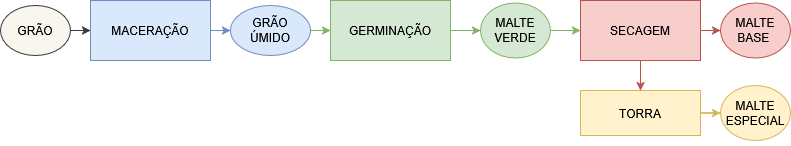
\includegraphics[width=1.0\textwidth]{fluxogramamalteacao.png}

    {\centering\footnotesize Fonte: Autoria própria.\par}
\end{figure}

\subsection{Maceração}

Durante a maceração, com a submersão do grão em água, ocorre a liberação de hormônios e enzimas que darão início ao crescimento e desenvolvimento do grão \cite{LEWIS2012}. O teor de água no grão cresce rapidamente após o início dessa primeira etapa, que ocorre em duas fases distintas: uma inicial, em que o embrião e o escutelo absorvem água rapidamente, e uma segunda fase, mais lenta, em que o endosperma é gradualmente hidratado. Esse processo é crucial para a ativação de enzimas como a amilase, a ribonuclease e a fosfatase, que desempenham papeis essenciais na modificação do grão \cite{REYNOLDS1966}. Também é crucial que o oxigênio seja fornecido ao mesmo tempo em que o dióxido de carbono é eliminado dos grãos. O aumento da umidade intensifica o metabolismo do grão, elevando sua taxa respiratória, ou seja, mais oxigênio é requerido \cite{KUNZE1996}. Por isso, a presença de tanques de maceração que bombeiam ar através dos grãos submersos é frequente nas produções de larga escala \cite{CENCI2021}. Mas, muitos estudos ainda investigam os impactos de se trabalhar com ciclos de períodos secos e submersos, especialmente, quando se busca viabilizar novas variedades de grãos para a malteação \cite{MAYER2014,TURNER2019}.

\begin{figure}[ht]
    \centering
    \caption{Estrutura do grão de cevada.}
    \label{fig:graodecevada}
    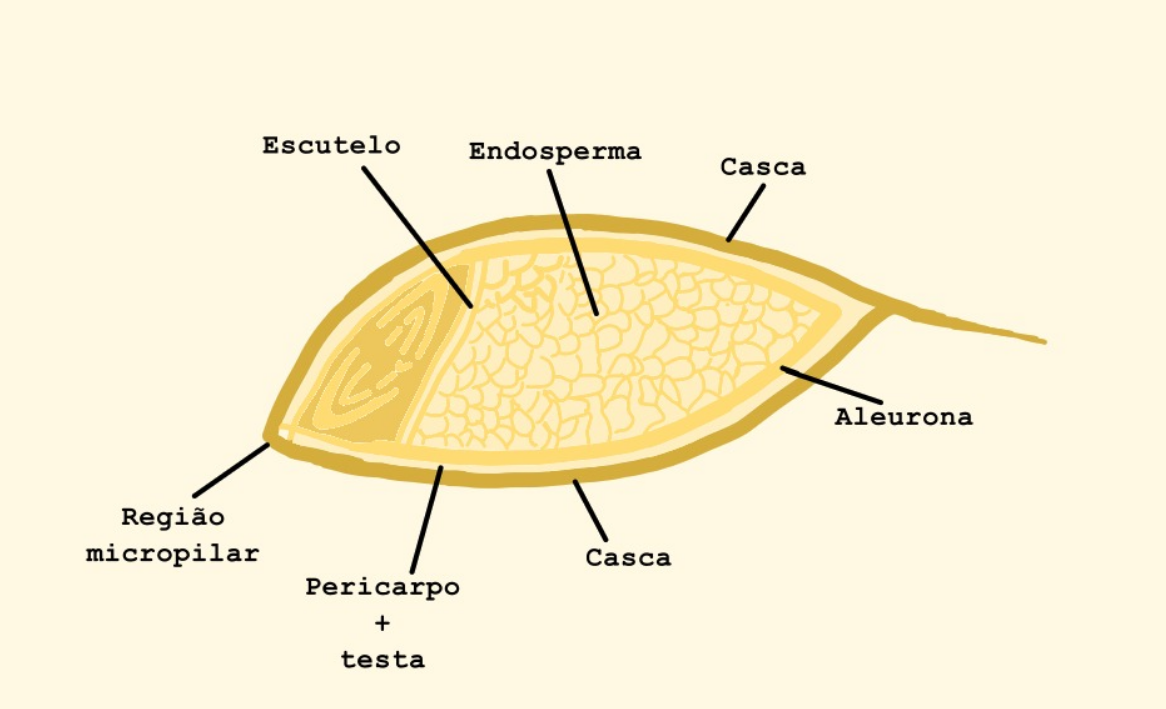
\includegraphics[width=0.9\textwidth]{graodecevada.png}

    {\centering\footnotesize Fonte: Autoria própria. Adaptado de \citeonline{LEWIS2012}.\par}
\end{figure}



\subsection{Germinação}

Ao fim da maceração, que pode durar até 72 horas, o teor de umidade dos grãos chega a aproximadamente 45\%, e as radículas tornam-se visíveis, indicando o momento adequado para o início da germinação. Essa segunda etapa é caracterizada por um elevado nível metabólico nos grãos, com a ocorrência de transformações bioquímicas essenciais para o processo de malteação \cite{MALLETT2022}. Do ponto de vista do malteador, a duração da germinação deve ser cuidadosamente controlada, pois um período insuficiente ou excessivo pode comprometer a qualidade do malte. Se a germinação for muito curta, as transformações necessárias nos grãos não ocorrerão de forma adequada. Por exemplo, as enzimas não conseguirão degradar completamente as paredes celulares proteicas que envolvem o amido, tornando-o menos disponível para as etapas subsequentes do processo cervejeiro \cite{FOX2009}. Por outro lado, uma germinação prolongada pode levar ao esgotamento excessivo dos nutrientes do grão visando o crescimento da planta, afetando negativamente o produto final \cite{LEWIS2012}.

Durante a germinação, a ativação de enzimas hidrolíticas desempenha um papel essencial na modificação do grão. As $\beta$-glucanases promovem a degradação dos $\beta$-glucanos (\autoref{fig:betaglucanos}) presentes na parede celular do endosperma, substâncias estas que são indesejadas no processo cervejeiro em altas concentrações \cite{LEWIS2012}. Essas enzimas hidrolisam as ligações $\beta$-1,3 e $\beta$-1,4 dos glucanos de cadeia mista, comprometendo a integridade da parede celular e facilitando a liberação de proteínas presentes nas células da camada de aleurona (\autoref{fig:graodecevada}) \cite{bobade2022betaglucans}. Paralelamente, proteases hidrolisam a matriz proteica que envolve os grânulos de amido, liberando pequenos peptídeos e aminoácidos \cite{FOX2009,GUPTA2010}. Já a conversão do amido (\autoref{fig:amido}) é mediada por enzimas amilolíticas, sendo a $\alpha$-amilase responsável pela quebra aleatória das ligações $\alpha$-1,4-glicosídicas e a $\beta$-amilase pela liberação de maltose, um dos principais açúcares fermentáveis do processo cervejeiro \cite{GUPTA2010,MALLETT2022}. Em essência, o grão cru entra no processo com compostos de alto peso molecular e, ao fim da malteação, gera como produto um malte com compostos de baixo peso molecular e boa concentração de enzimas \cite{KUNZE1996}. Essa transformação, que ocorre principalmente na germinação, é o que torna o malte indispensável para o processo cervejeiro \cite{CENCI2021}.

\begin{figure}[ht]
    \centering
    \caption{Esquema de uma molécula de $\beta$-glucano.}
    \label{fig:betaglucanos}
    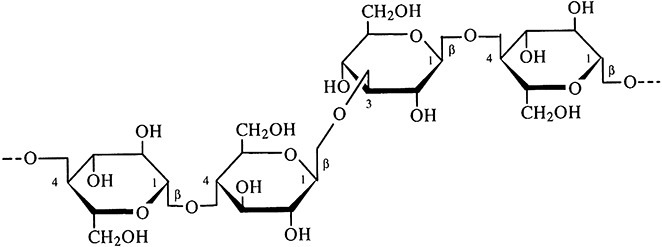
\includegraphics[width=0.9\textwidth]{betaglucanos.jpg}

    {\centering\footnotesize Fonte: \citeonline{rop2009betaglucans}.\par}
\end{figure}

\begin{figure}[ht]
    \centering
    \caption{Estrutura química do amido representando as unidades de amilose (\textit{amylose}) e amilopectina (\textit{amylopectin}).}
    \label{fig:amido}
    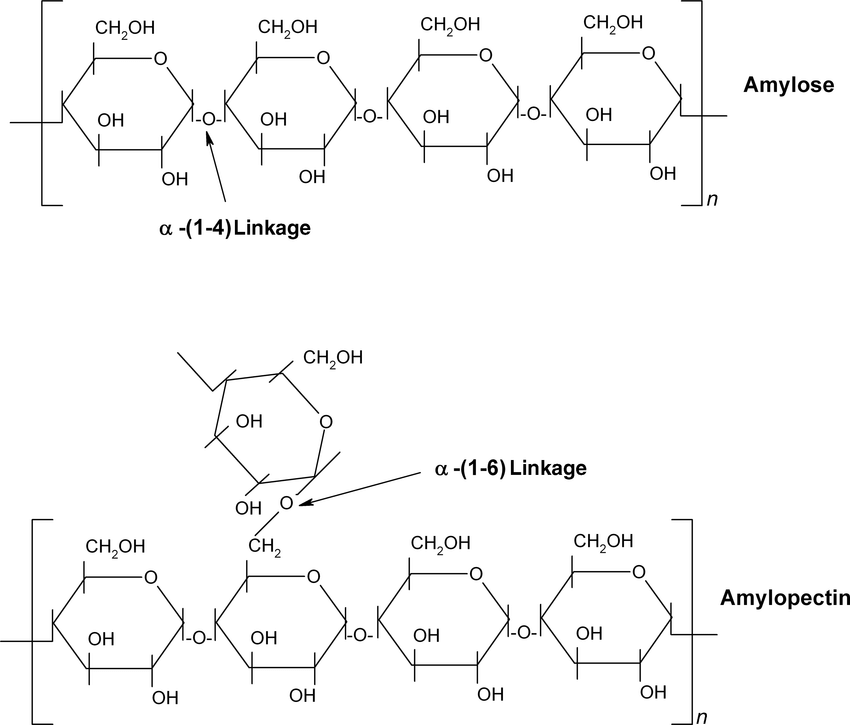
\includegraphics[width=0.9\textwidth]{amido.png}

    {\centering\footnotesize Fonte: \citeonline{visakh2012starch}.\par}
\end{figure}

\begin{table}[ht]
    \caption{Comparativo entre as enzimas $\alpha$-amilase e $\beta$-amilase.}
    \label{tab:amilases}
    \centering
    \begin{tabular}{ccc}
        \hline
        \bfseries Característica & \bfseries $\alpha$-amilase & \bfseries $\beta$-amilase \\
        \hline
        Posição de ataque & Interna na cadeia & Extremos não redutores \\
        Produto principal & Maltose, glicose e dextrinas & Maltose \\
        Ligação hidrolisada & $\alpha$-1,4 & $\alpha$-1,4 \\
        Temperatura ideal & 70 -- 75 $^{\circ}$C & 60 -- 65 $^{\circ}$C \\
        Termoestabilidade & Alta & Moderada \\
        Papel no processo & Liquefação do amido & Produção de açúcares fermentáveis \\
        \hline
    \end{tabular}

    {\centering\footnotesize Fonte: Adaptado de \citeonline{GUPTA2010}, \citeonline{LEWIS2012}, \citeonline{MALLETT2022}.\par}
\end{table}



\subsection{Secagem}

Quando a germinação atinge o tempo otimizado para promover as melhores transformações, inicia-se a etapa de secagem. Nessa fase, de acordo com \apudonline{GRIFFITHS1992}{WOFFENDEN2002}, os grãos são desidratados por até 30 horas, o que resulta em um malte base de fácil manuseio e adequado para armazenamento. Além da redução da umidade para aumento da estabilidade do produto final, a secagem promove o desenvolvimento de aromas desejados e de coloração no malte \cite{BAMFORTH2003}. Apesar disso, se a intenção é produzir um malte base, a temperatura não pode ser excessiva, com o fim de preservar as enzimas, como as amilases, no produto final \cite{LEWIS2012}.Outra questão benéfica é que a secagem elimina boa parte dos microorganismos que cresceram de forma indesejada durante os processos anteriores \cite{DOUGLAS1988, PETTERS1988}. 



\section{Variáveis na malteação}

\subsection{Temperatura}

O controle da temperatura durante a germinação é essencial para minimizar perdas causadas pelo crescimento excessivo das radículas e do embrião da planta, evitando o consumo desnecessário dos estoques de amido do grão \cite{PITZ1990, MALLETT2022}. Além disso, a temperatura influencia diretamente a atividade enzimática e a degradação de componentes estruturais do grão. Um estudo conduzido por \citeonline{BAXTER1980} avaliou os efeitos da maceração em uma temperatura superior à faixa usual de 12-16 $^{\circ}$C, chegando a 30 $^{\circ}$C. Os resultados indicaram que temperaturas elevadas comprometem a atividade enzimática e reduzem a eficiência da degradação de $\beta$-glucanos e proteínas, afetando negativamente a qualidade do malte.

Outro fator crítico relacionado à temperatura é o crescimento microbiológico. Segundo \citeonline{TANGNI2002}, temperaturas mais altas na malteação favorecem a proliferação de \textit{Aspergillus clavatus}, um fungo produtor de micotoxinas. A contaminação microbiológica ocorre predominantemente durante a germinação, mas também pode ser observada ao final da maceração \cite{PETTERS1988}. Dessa forma, a manutenção de temperaturas controladas entre 12 e 22 $^{\circ}$C durante as etapas de maceração e germinação é fundamental não apenas para garantir a qualidade do malte, mas também para assegurar a segurança sanitária do processo \cite{TANGNI2002}.

\subsubsection{Temperatura na secagem}

Na etapa de secagem, o controle da temperatura desempenha um papel crucial em dois aspectos principais: garantir que o malte atinja a umidade adequada para armazenamento e determinar o tipo de malte produzido \cite{KUNZE1996}. A secagem ocorre, geralmente, em múltiplas fases, seguindo uma rampa de temperatura. Os valores típicos variam na faixa de 50 a 110 $^{\circ}$C, dependendo do perfil desejado para o malte final \cite{LEWIS2012}.

De acordo com \citeonline{SKENDI2018}, a temperatura de secagem influencia diretamente a composição de açúcares fermentáveis no malte e a coloração do mosto produzido. No estudo, a secagem a 80 $^{\circ}$C resultou em um mosto com maior teor de açúcares fermentáveis do que a secagem a temperaturas superiores, como 90 $^{\circ}$C. Além disso, foi observado um escurecimento do mosto com o aumento da temperatura de secagem, um fator determinante na definição das características finais do malte. Essa relação entre temperatura e cor ocorre devido à intensificação das reações de Maillard e à degradação térmica de compostos presentes no malte \cite{KUNZE1996}.

\subsection{Aeração}

A aeração dos grãos é um aspecto essencial da malteação, uma vez que o processo envolve um organismo vivo que depende da respiração para seu desenvolvimento \cite{MALLETT2022}. De acordo com \citeonline{WILHELMSOM2006}, no início da maceração ocorre uma deficiência de oxigênio devido à submersão dos grãos, mas esse fator não compromete a qualidade do malte. No entanto, à medida que a germinação avança, a disponibilidade de O$_2$ torna-se mais crítica, pois a respiração dos grãos gera acúmulo de dióxido de carbono, o que pode inibir a germinação. Esse efeito pode ser intensificado pelo emaranhamento das radículas, que dificulta a circulação de ar e reduz ainda mais a disponibilidade de oxigênio. Para mitigar esse problema, sistemas revolvedores são frequentemente empregados para movimentar os grãos e garantir uma aeração adequada ao longo do processo \cite{CENCI2021}. 

\subsection{Tempo}
A duração de cada etapa da malteação é um fator crítico para a qualidade do malte, influenciada pela variedade do grão e pelas condições do processo (umidade, temperatura e aeração). A otimização desse parâmetro é essencial para adaptar novas variedades às demandas industriais. Como demonstrado por \citeonline{FARNAZEH2017}, o tempo de germinação (3 a 7 dias) afeta diretamente as propriedades do malte: períodos mais longos (7 dias) elevam a atividade de $\beta$-glucanase e $\alpha$-amilase, reduzindo o teor de amido e $\beta$-glucano devido ao consumo enzimático, além de aumentar as perdas por crescimento. Assim, a definição do tempo ideal deve equilibrar modificação enzimática e eficiência do processo, considerando o perfil desejado no malte. Por exemplo, germinação prolongada é indicada para cervejas de alta fermentabilidade, enquanto períodos mais curtos (3-5 dias) preservam polissacarídeos, sendo ideais para estilos encorpados.

Na etapa de maceração, o tempo necessário para a hidratação dos grãos é um fator determinante para a ativação enzimática e o desenvolvimento adequado do malte. \citeonline{MONTANUCI2017} demonstraram que períodos mais longos de maceração favorecem a absorção de água, impactando diretamente a degradação de $\beta$-glucanos e o desenvolvimento das enzimas $\alpha$- e $\beta$-amilase. No entanto, o tempo ideal depende da temperatura empregada: enquanto macerações a 10 $^{\circ}$C por 24 horas resultam em maior teor de açúcares no malte, temperaturas mais elevadas (20 $^{\circ}$C por 12 horas) aceleram a hidratação, porém podem comprometer a viabilidade dos grãos e aumentar a degradação de componentes essenciais. Além disso, tempos excessivos de maceração podem favorecer o crescimento microbiológico indesejado, exigindo um controle rigoroso para evitar contaminações e perdas na qualidade do malte \cite{LUARASI2016}. Dessa forma, a definição do tempo de maceração deve equilibrar a eficiência da hidratação com a preservação da integridade dos grãos, garantindo um substrato adequado para as etapas subsequentes da malteação.

O tempo de secagem deve ser ajustado em conjunto com a temperatura para garantir uma remoção eficiente da umidade, reduzindo-a para aproximadamente 4\%, sem comprometer a qualidade enzimática e sensorial do malte \cite{LEWIS2012}.



\section{Automação e controle de processos}

A automação desempenha um papel essencial na indústria no geral, proporcionando maior qualidade no produto final, otimização da produção e aumento da segurança operacional \cite{SEBORG2016}. Para garantir um controle eficaz dos processos industriais, são utilizados sistemas instrumentados, compostos por três elementos fundamentais: sensores, processadores de sinais e interfaces de visualização \cite{BOLTON2021}. Os sensores são responsáveis pela coleta de informações sobre variáveis do processo, como temperatura, pressão e vazão, permitindo o monitoramento contínuo das condições operacionais. Os processadores de sinais, por sua vez, realizam o tratamento e a interpretação dos dados captados, aplicando algoritmos de controle para ajustar automaticamente os parâmetros do sistema conforme necessário. Já as interfaces de visualização possibilitam que operadores e engenheiros acompanhem o comportamento do processo em tempo real, viabilizando a tomada de decisões informadas e a rápida identificação de falhas \cite{BOLTON2021}. Além disso, sistemas automatizados contribuem significativamente para a reprodutibilidade dos processos industriais, reduzindo variações indesejadas e garantindo conformidade com padrões regulatórios \cite{SEBORG2016}.

\subsection{Controlador ON-OFF}
O controlador ON-OFF é um dos métodos mais simples de controle de processos, operando com apenas dois estados: ligado (ON) e desligado (OFF). Esse tipo de controle é amplamente utilizado quando precisão extrema não é necessária e o sistema pode tolerar pequenas oscilações na variável controlada \cite{BOLTON2021}. Seu funcionamento é baseado em um ponto de ajuste (setpoint): quando a variável de processo ultrapassa esse valor, o atuador é ativado ou desativado, sem intermediários. Embora seja uma solução de fácil implementação e baixo custo, pode gerar oscilações constantes em torno do setpoint, tornando-se inadequado para processos que exigem estabilidade mais refinada \cite{SEBORG2016}.

\subsection{Interfaces Gráficas (GUI)}
A Interface Gráfica do Usuário (GUI) é um elemento essencial na automação, pois permite a interação intuitiva entre operadores e sistemas de controle. Segundo \citeonline{BOLTON2021}, esse tipo de interface apresenta informações de processo de forma visual e interativa, utilizando janelas, ícones, menus e dispositivos apontadores (WIMP - Windows, Icons, Menus, Pointing Device). Em ambientes industriais, as telas de supervisão geralmente empregam displays miméticos, que representam esquematicamente as principais partes de uma planta, exibindo valores atualizados de variáveis controladas, gráficos de tendências e alarmes em tempo real. Além disso, as interfaces gráficas possibilitam que os operadores definam valores de setpoint e ajustem parâmetros do processo diretamente pela tela, eliminando a necessidade de comandos textuais complexos.



\section{ESP32}

O ESP32 é uma evolução do ESP8266, apresentando melhorias significativas, como suporte a Bluetooth dual-mode (Classic e Low Energy) e Wi-Fi integrado, além de um processamento mais robusto e maior eficiência energética \cite{TOLLERVEY2017}.

De acordo com \citeonline{KOLBAN2017}, os circuitos integrados baseados no ESP32 são amplamente utilizados devido ao seu baixo custo e à capacidade de executar aplicações autônomas, tornando-se uma escolha popular para projetos de automação e controle de processos. Além disso, sua versatilidade permite a integração com diversos sensores e dispositivos periféricos, tornando-o adequado para uma ampla gama de aplicações em automação e sistemas embarcados.

Graças à sua conectividade com a internet, as placas ESP32 estão fortemente associadas ao conceito de Internet das Coisas (IoT). O IoT tem papel fundamental na otimização de processos industriais, permitindo a coleta de dados em larga escala (big data) e a detecção de falhas, o que contribui para a redução de custos operacionais \cite{ferencz2020rapid}. Essa tecnologia é composta por uma variedade de dispositivos, como sensores, atuadores e controladores, que podem se comunicar por meio de diferentes protocolos, incluindo Bluetooth, Ethernet e Wi-Fi \cite{shinde2017industrial}.

Um exemplo prático do uso do IoT em aplicações industriais foi apresentado por \citeonline{shinde2017industrial}, que desenvolveram um sistema de monitoramento de energia utilizando o ESP8266 Wi-Fi. Nesse estudo, os dados coletados eram processados e exibidos em uma interface web, demonstrando a viabilidade da automação industrial baseada em IoT.


\subsection{MicroPython}

O MicroPython é um interpretador da linguagem Python 3 desenvolvido especificamente para microcontroladores \cite{PLAUSKA2022}. A linguagem Python destaca-se por sua sintaxe simplificada e ampla adoção na comunidade tecnológica, sendo especialmente útil para programadores iniciantes \cite{TOLLERVEY2017}.

Estudos conduzidos por \citeonline{PLAUSKA2022} avaliaram o desempenho das principais linguagens utilizadas na programação do ESP32, incluindo o MicroPython. Os resultados indicaram que, embora sua eficiência em termos de desempenho seja inferior à de linguagens compiladas, como C e C++, o MicroPython continua sendo uma alternativa viável para aplicações em sistemas de alto nível. Sua principal vantagem reside na facilidade de prototipação e desenvolvimento rápido, tornando-o ideal para projetos onde o controle fino do hardware não é um requisito crítico \cite{tanganelli2019rapid}.



\section{Android}

O Android é um dos principais sistemas operacionais para dispositivos móveis, sendo um projeto de código aberto baseado no kernel Linux e liderado pelo Google \cite{ABLESON2011}. Inicialmente, os aplicativos desenvolvidos para essa plataforma eram escritos predominantemente em Java \cite{ABLESON2011}. No entanto, em 2017, o Google anunciou suporte oficial ao Kotlin como linguagem de desenvolvimento para Android \cite{SILLS2023}.

A integração entre sistemas IoT e dispositivos móveis baseados em Android é um avanço importante para aplicações de monitoramento remoto. Um exemplo desse tipo de integração foi descrito por \citeonline{mohanasundaram2024water}, que desenvolveram um sistema para monitoramento da qualidade da água em tempo real. O sistema utilizava sensores de pH, turbidez, temperatura e nível de água para coletar dados, que eram então disponibilizados para visualização em uma aplicação Android e em uma interface web, permitindo o acesso remoto, também, a partir de outros sistemas operacionais. Segundo os autores, o uso da automação e da tecnologia embarcada promovida pelo IoT simplificou significativamente o processo de coleta de dados, aumentando a eficiência e a precisão na avaliação da qualidade da água.

\subsection{Kotlin}

O Kotlin se destaca como uma linguagem moderna, concisa, segura e pragmática, oferecendo total interoperabilidade com código Java, o que facilita a migração e a integração de projetos legados \cite{JEMEROV2017}. Atualmente, é amplamente adotado como a principal linguagem para o desenvolvimento de aplicativos móveis na plataforma Android, proporcionando maior produtividade e reduzindo a incidência de erros comuns durante a programação.

\subsection{Bluetooth}

A plataforma Android oferece suporte a diferentes protocolos de comunicação via Bluetooth, incluindo o Bluetooth Low Energy (BLE), possibilitando a conexão eficiente com dispositivos como o ESP32 \cite{android_bluetooth_overview}.

O BLE foi desenvolvido como uma extensão do Bluetooth clássico, com o objetivo de reduzir significativamente o consumo de energia sem comprometer a conectividade \cite{heydon2012bluetooth}. Essa tecnologia é utilizada em aplicações que exigem comunicação contínua com baixo consumo energético. No contexto da automação e do monitoramento remoto, a integração entre Android e ESP32 via BLE permite a troca eficiente de dados em tempo real, viabilizando aplicações que demandam conectividade sem a necessidade de conexões Wi-Fi ou a cabo.

% Talvez falar sobre Git e GitHub dependendo dos resultados...